\begin{frame}{Content}
    \begin{enumerate}%
      \setlength\itemsep{1em}%
      \item {\color{lightgray} \ti{}} \tei{}
      \item {\color{lightgray} \tii{}} \teii{}
      \item {\color{lightgray} \tciii{}} \teiii{}
      \item {\color{lightgray} \tiv{}} \teiv{}
      \item {\color{lightgray} \tv{}} \tev{}
      \item {\color{lightgray} \tvi{}} \tevi{}
    \end{enumerate}
  \end{frame}

\begin{frame}{\tciii{} A Geometric Encoding for Neural Network Evolution}
    
    \begin{columns}
    \begin{column}{0.45\linewidth}
    \begin{center}
        \onslide<2->{
        \begin{figure}
        \centering
        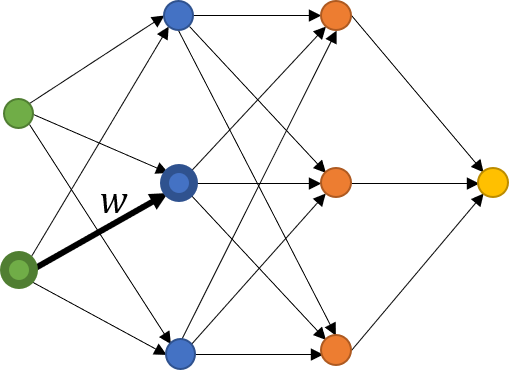
\includegraphics[height=.7\linewidth]{images/GENE/images/gene_graph.png}
        \end{figure}
        }
    \end{center}
    \end{column}
    
    \begin{column}{0.45\linewidth}
    \begin{center}
        \onslide<3->{
        \begin{figure}
        \centering
        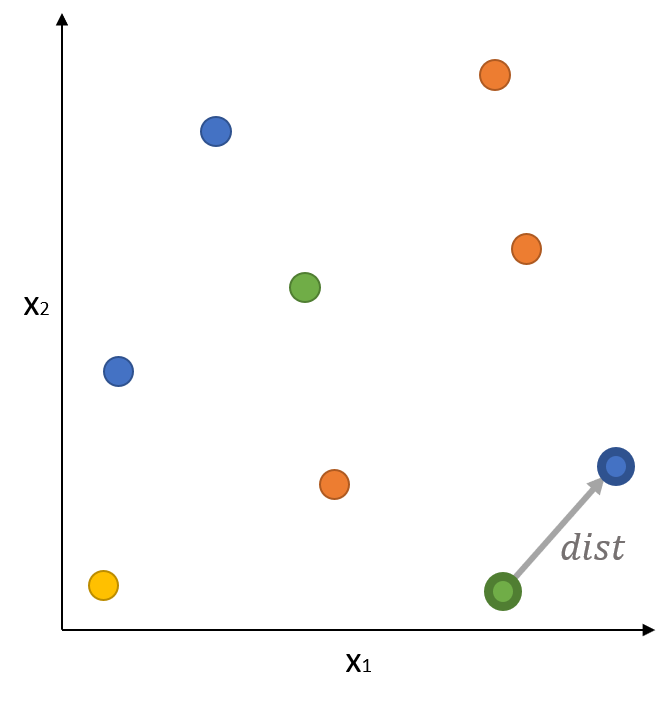
\includegraphics[height=.8\linewidth]{images/GENE/images/gene_coordinates.png}
        \end{figure}
        }
    \end{center}
    \end{column}
    \end{columns}
    
    \begin{columns}
    \begin{column}{0.45\linewidth}
    \begin{center}
        \onslide<2->{
        Fully connected \\ neural network
        }
    \end{center}
    \end{column}
    
    \begin{column}{0.45\linewidth}
    \begin{center}
        \onslide<3->{
            GENE encoding \\ {\color{lightgray} \cite{templierGeometricEncodingNeural2021}}
        }
    
    \end{center}
    \end{column}
    \end{columns}
    
\end{frame}


% L2 and signed
\begin{frame}{\tciii{} \gene: Distance functions}
    \begin{equation}
    w_{i, j} = dist(n_i, n_j)
    \end{equation}
    
    \begin{columns}
    \begin{column}{0.60\linewidth}
    \begin{block}{Euclidean distance}
    \begin{equation}
    \sqrt{\sum_{k=1}^D \left( n_1^k - n_2^k \right)^2 }
    \end{equation}
    \end{block}
    \end{column}
    
    \begin{column}{0.35\linewidth}
    \begin{figure}
    \centering
    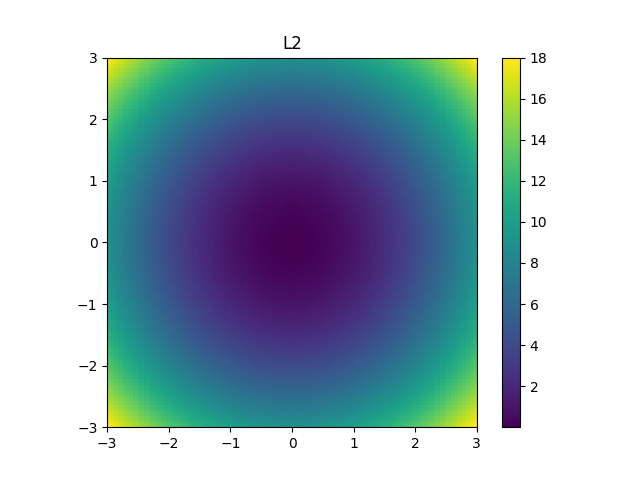
\includegraphics[width=\linewidth]{images/GENE/images/distance_L2.png}
    \end{figure}
    \end{column}
    \end{columns}
    
    % \begin{block}{Euclidean distance}
    
    % \end{equation}
    % \end{block}
    
\end{frame}

% Weights
\begin{frame}{\tciii{} \gene: Weight distribution}
    
    \begin{figure}
    \centering
    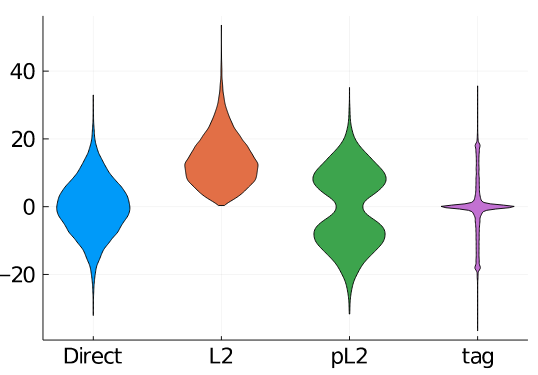
\includegraphics[width=.7\linewidth]{images/GENE/images/weights_distrib.png}
\end{figure}
\begin{center}
    \small Distribution of weight values in networks evolved with different encodings.
\end{center}
\end{frame}

\begin{frame}{\tciii{} Experimental setup}
\begin{columns}
        
    \begin{column}{0.7\linewidth}
    \begin{center}
        \begin{figure}
        \centering
        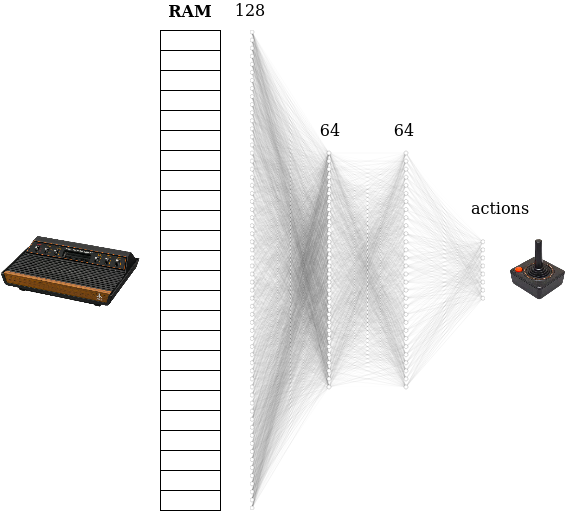
\includegraphics[width=.7\linewidth]{images/GENE/images/RAM_net.png}
        \small \\ RAM state representation
          \end{figure}
    
    \end{center}
    \end{column}
    
    \begin{column}{0.3\linewidth}
    \begin{center}
    \onslide<2->{
        \begin{block}{SNES}
            \begin{itemize}
                \item Separable NES 
                \item Complexity in $O(n)$
            \end{itemize}
        \end{block}

        \begin{block}{XNES}  
            \begin{itemize}
                \item Exponential NES
                \item Complexity in $O(n^2)$
            \end{itemize}
        \end{block}
    }
    \onslide<3->{
        \begin{block}{Encodings}  
            \begin{itemize}
                \item Direct encoding
                \item GENE: dim=3
                \item 10 runs
            \end{itemize}
        \end{block}
    }
    \end{center}
    \end{column}

    \end{columns}
\end{frame}


% Update step
\begin{frame}{\tciii{} Computational cost}
    
    \begin{block}{Evolutionary Strategy update of $\mu$ and $\sigma$} 
            \begin{table}
                \begin{tabular}{llllrr}
                        Encoding  & $D$ & Genes &  &  Mean time (s) &  Memory (KiB) \\
                    \midrule
                    \pltwogene{} &   3 & 804 & SNES &       0.000357 &                 630.56 \\
                    \pltwogene{} &  10 & 2211 & SNES &       0.000678 &                1372.16 \\
                     Direct &   - & 5609 & SNES &       0.001350 &                3133.44 \\
                    \pltwogene{} &   3 & 804 & XNES &       1.475000 &             1352663.04 \\
                    \pltwogene{} &  10 & 2211 & XNES &      14.244000 &            11806965.76 \\
                     Direct &   - & 5609 & XNES &     119.976000 &            79765176.32 \\
                    \end{tabular}
    %            \caption{Average time and memory for the build step of 1 individual, for a 128-32-32-9 network. All \coordsnet{} functions have similar build time, so only \pltwogene{} is used.}
            \end{table}
        \end{block}
    \end{frame}


% Results
\begin{frame}{\tciii{} Competitive results - Arcade Learning Environment}
    \onslide<1->{
    %SpaceInvaders
    \begin{columns}
      \begin{column}{0.45\linewidth}
        \begin{center}
          \begin{figure}
              \centering
              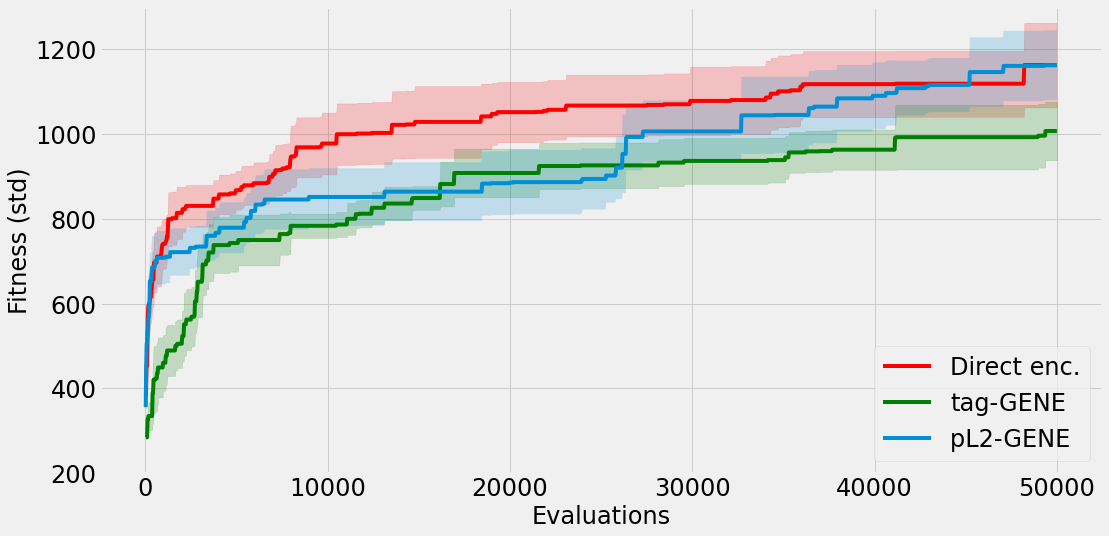
\includegraphics[width=.9\linewidth]{images/GENE/plots/SpaceInvaders - 128-64-64-6 - snes.png}
        \small SNES on SpaceInvaders
          \end{figure}
        \end{center}
      \end{column}
      
      \begin{column}{0.45\linewidth}
        \begin{center}
          \begin{figure}
              \centering
   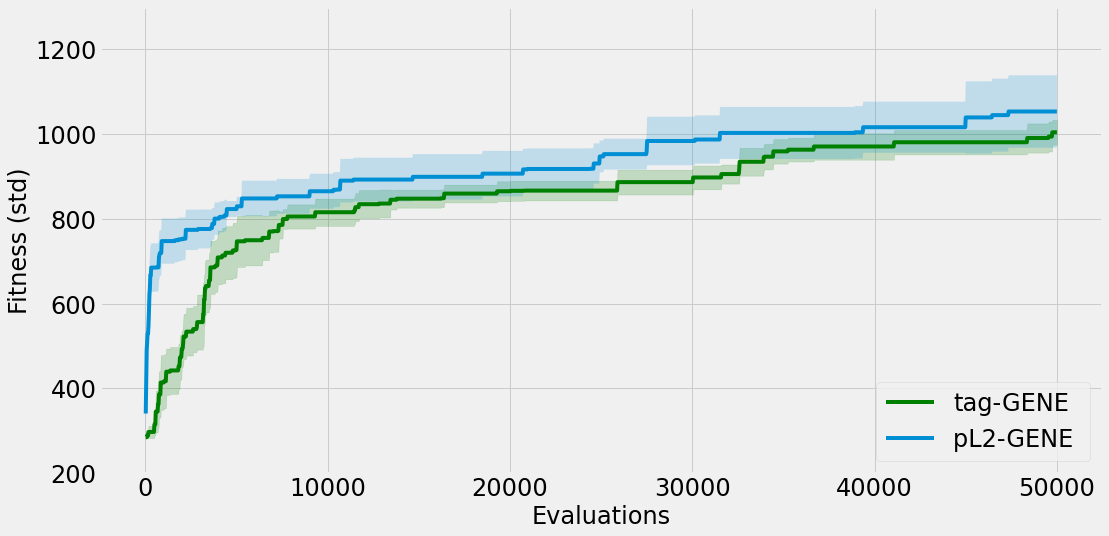
\includegraphics[width=.9\linewidth]{images/GENE/plots/SpaceInvaders - 128-64-64-6 - xnes.png}
        \small XNES on SpaceInvaders
          \end{figure}
        \end{center}
      \end{column}
    \end{columns}
    }

    \onslide<2->{
    % Seaquest
     \begin{columns}
      \begin{column}{0.45\linewidth}
        \begin{center}
          \begin{figure}
              \centering
              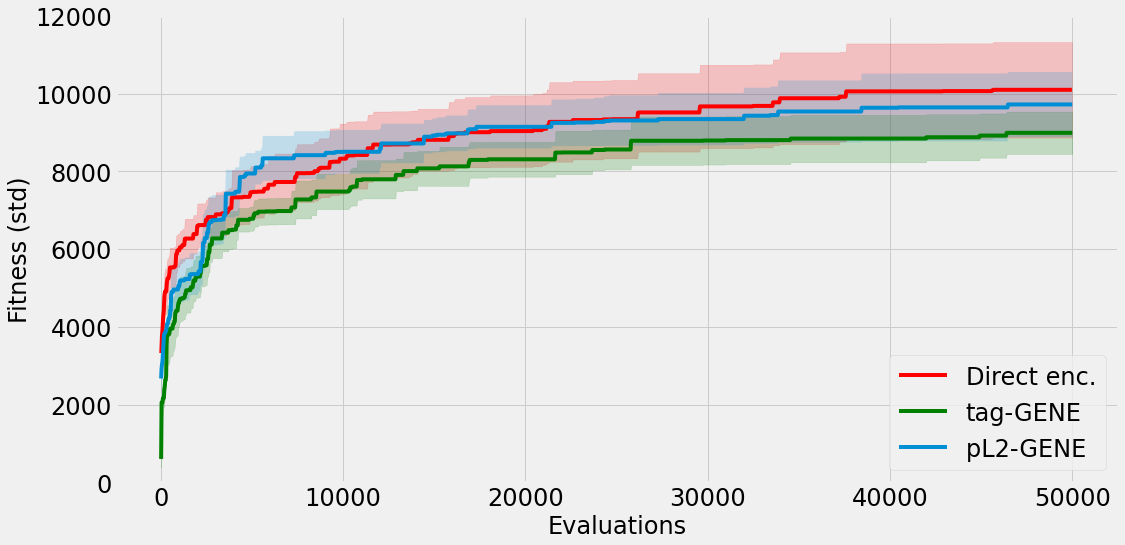
\includegraphics[width=.9\linewidth]{images/GENE/plots/krull - 128-64-64-18 - snes.png}
        \small SNES on Krull
          \end{figure}
        \end{center}
      \end{column}
      
      \begin{column}{0.45\linewidth}
        \begin{center}
          \begin{figure}
              \centering
   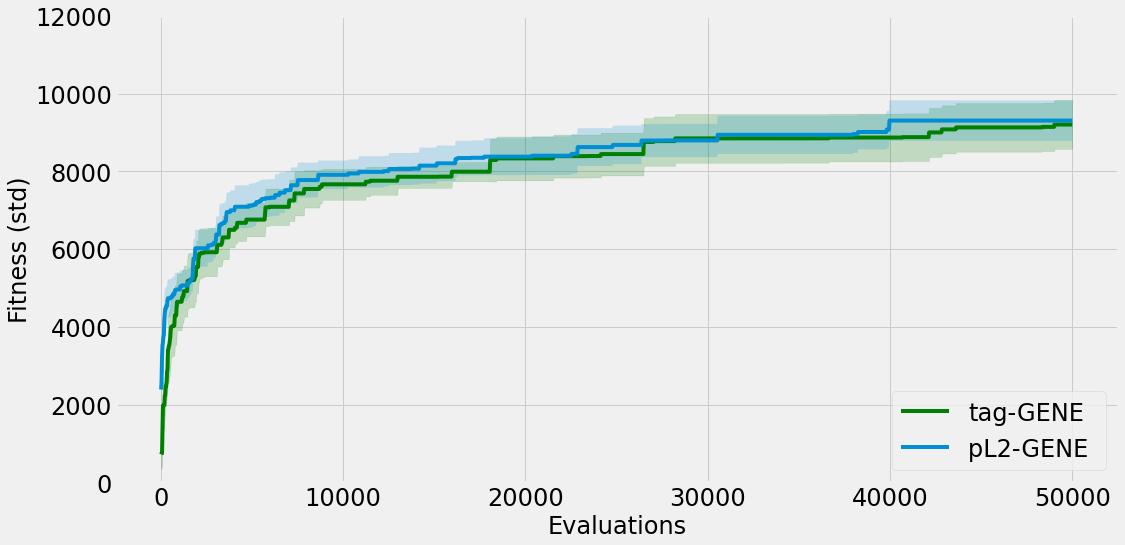
\includegraphics[width=.9\linewidth]{images/GENE/plots/krull - 128-64-64-18 - xnes.png}
        \small XNES on Krull
          \end{figure}
        \end{center}
      \end{column}
    \end{columns}
    }
  
  \end{frame}
  
  % Results
  \begin{frame}{\tciii{} Improving results - Arcade Learning Environment}
    \onslide<1->{
    %IceHockey
    \begin{columns}
      \begin{column}{0.45\linewidth}
        \begin{center}
          \begin{figure}
              \centering
              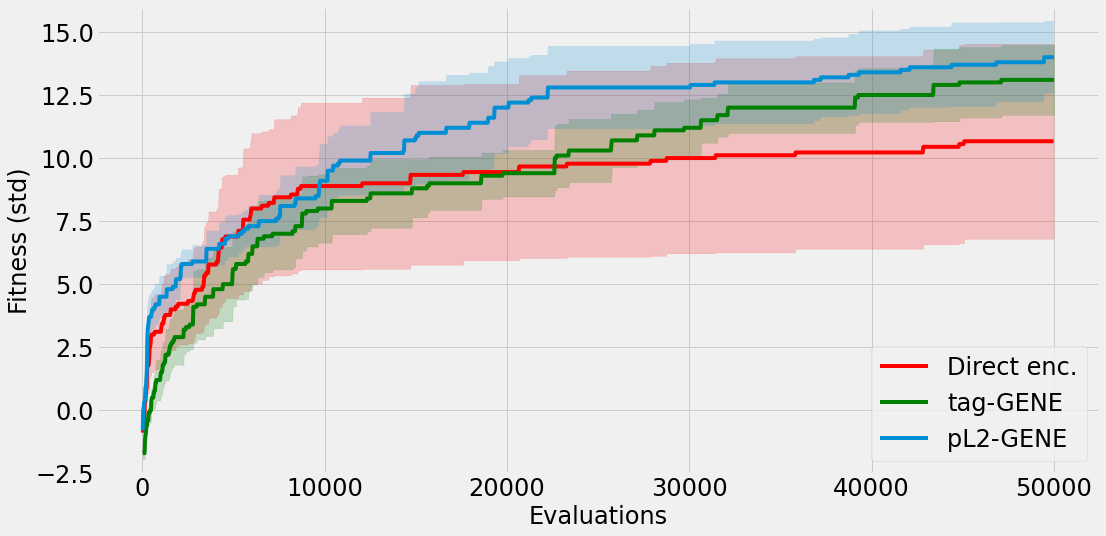
\includegraphics[width=.9\linewidth]{images/GENE/plots/IceHockey - 128-64-64-18 - snes.png}
        \small SNES on IceHockey
          \end{figure}
        \end{center}
      \end{column}
      
      \begin{column}{0.45\linewidth}
        \begin{center}
          \begin{figure}
              \centering
   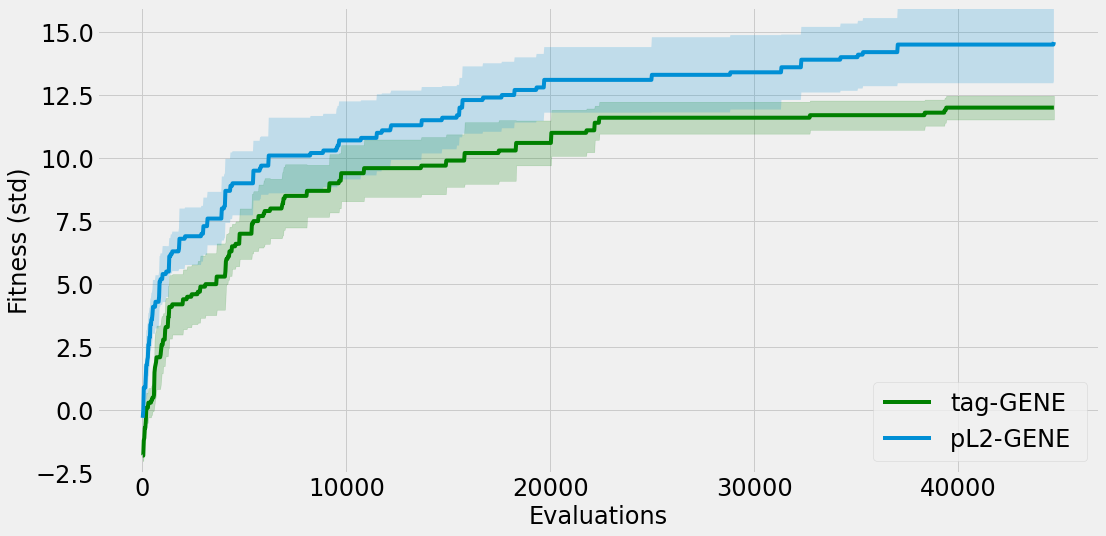
\includegraphics[width=.9\linewidth]{images/GENE/plots/IceHockey - 128-64-64-18 - xnes.png}
        \small XNES on IceHockey
          \end{figure}
        \end{center}
      \end{column}
    \end{columns}
    }
    \onslide<2->{
    % Seaquest
     \begin{columns}
      \begin{column}{0.45\linewidth}
        \begin{center}
          \begin{figure}
              \centering
              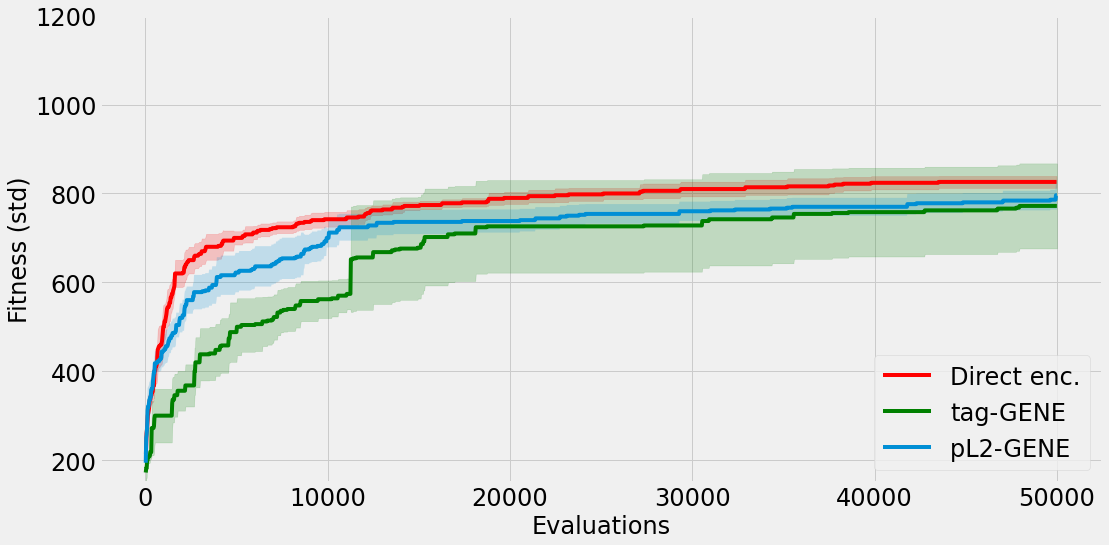
\includegraphics[width=.9\linewidth]{images/GENE/plots/seaquest - 128-64-64-18 - snes.png}
        \small SNES on Seaquest
          \end{figure}
        \end{center}
      \end{column}
      
      \begin{column}{0.45\linewidth}
        \begin{center}
          \begin{figure}
              \centering
   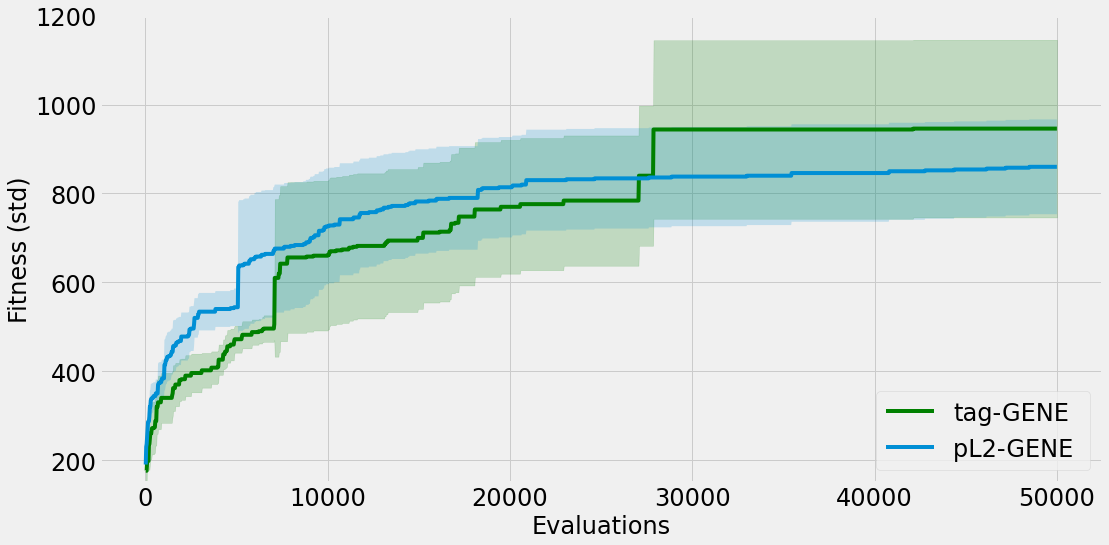
\includegraphics[width=.9\linewidth]{images/GENE/plots/seaquest - 128-64-64-18 - xnes.png}
        \small XNES on Seaquest
          \end{figure}
        \end{center}
      \end{column}
    \end{columns}
    }
  \end{frame}
  
  
  \begin{frame}{\tciii{} \fw}
    
    \begin{columns}
    \begin{column}{0.45\linewidth}
    \begin{center}
    \begin{block}{Distance functions}
    Design new distance functions, or optimize them through co-evolution.
    \end{block}
    
    \begin{block}{Hybrid encoding}
    Switch between indirect and direct encodings during the evolution.
    \end{block}
    \end{center}
    \end{column}
    
    \begin{column}{0.45\linewidth}
    \begin{center}
    \begin{block}{Gradient descent}
    Use backpropagation and gradient descent to optimize genomes instead of evolution.
    \end{block}
    
    \begin{block}{Complex networks}
    Design encodings for convolution layers and recurrent networks.
    \end{block}
    \end{center}
    \end{column}
    \end{columns}
    
    \end{frame}